\documentclass[a4paper,french,bookmarks]{article}
\usepackage{./Structure/4PE18TEXTB}

\renewcommand{\thesection}{\Roman{section}.}

%fonctions de Jacobi
\funlvi{am}
\funlvi{sn}
\funlvi{cn}
\funlvi{dn}
\begin{document}
\stylize{Mathématiques}{Devoir Maison 9 : Jacobi et le pendule simple}

Soit $k$ un réel tel que $k \in [0, 1[$.
\section{Fonction amplitude de Jacobi}

\begin{enumerate}
    \item Montrer que la fonction $f : t \mapsto \dfrac{1}{\sqrt{1-k^2\sin^2 t}}$ est définie et continue sur $\bdR$.
    
     \boxans{
        Soit $t \in \bdR$. On a $-1 \leq \sin t \leq 1$ donc $\sin^2 t \leq 1$. Avec $k \in [0, 1[$, on a donc $k^2\sin^2 t < 1$.
        
        Donc $1 - k^2\sin^2 t > 0$, et donc $\sqrt{1 - k^2\sin^2 t} > 0$. 
        
        Puisque le dénominateur de $f$ ne s'annule jamais sur $\bdR$, \boxsol{la fonction $f$ est toujours définie sur $\bdR$}.
        
        Or $f$ est une composée de fonctions continues, donc \boxsol{la fonction $f$ est continue sur $\bdR$}
     }
\end{enumerate}

On peut alors poser pour tout réel $x$ la fonction $A$ définie par :
\[ A(x) = \int_0^x \dfrac{\dif t}{\sqrt{1-k^2\sin^2 t}} \qquad \text{et} \qquad K=A\left(\dfrac{\pi}{2}\right)\]
\begin{enumerate}[resume]
    \item \begin{enumerate}
        \item Montrer que $A$ est dérivable et strictement croissante sur $\bdR$.
        
        \boxans{
        On remarque que $\forall x \in \bdR$, $\displaystyle A(x) = \int_0^x f(t)\dif t$. Le théorème fondamental de l'analyse livre alors que $A$ est une primitive de $f$ sur $\bdR$, donc \boxsol{$A$ est dérivable sur $\bdR$} de dérivée $f$. 
        
        Or $\forall x \in \bdR$, $A'(x)=f(x)=\dfrac{1}{\sqrt{1-k^2\sin^2x}} > 0$. Donc \boxsol{$A$ est strictement croissante sur $\bdR$}.
        }
        
        \item Montrer que pour tout réel positif $x$, \quad $A(x) \geq x$. \qquad En déduire la limite de $A$ en $+\infty$.
        
        \boxans{
        Soit $x \in \bdR_+$ et $t \in [0, x]$. On a $0 < \sqrt{1 - k^2\sin^2t} \leq 1$ donc $\dfrac{1}{\sqrt{1-k^2\sin^2t}} \geq 1$.
        
        Par préservation de l'ordre $\forall x \in \bdR_+$, $\displaystyle \int_0^x \dfrac{\dif t}{\sqrt{1-k^2\sin^2t}} \geq \int_0^x \dif t$, donc \boxsol{$\forall x \in \bdR_+$, $A(x) \geq x$}.
        
        De plus, $\lim\limits_{x \to +\infty} x = +\infty$ donc par théorème de minoration \boxsol{$\lim\limits_{x \to +\infty} A(x) = +\infty$}.
        }
        
        \item  Étudier la parité/imparité de $A$.
        \boxans{
        Soit $x \in \bdR$. On remarque que $f$ est paire puisque 
        \[f(-t) = \dfrac{1}{\sqrt{1-k^2\sin^2 (-x)}} = \dfrac{1}{\sqrt{1-k^2\left(-\sin x\right)^2}} = \dfrac{1}{\sqrt{1-k^2\sin^2 x}} = f(t)\]
        
        On a $A(-x) = \displaystyle \int_0^{-x} f(t)\dif t$. On pose le changement de variable $t = -u$, donc $\dif t = -\dif u$. On a donc :
        \[A(-x) = \int_0^{x} f(-u)(-\dif u) = -\int_0^{x} f(u)\dif u = -A(x) \qquad \text{donc} \ \boxsol{la fonction $A$ est impaire}.\]
        }

        \item  Montrer que $A$ est bijective de $\bdR$ dans $\bdR$.
        
        \boxans{
        $A$ est impaire, et $\lim\limits_{x \to +\infty} A(x) = +\infty$ donc $\lim\limits_{x \to -\infty} A(x) = -\infty$. $A$ est strictement croissante sur $\bdR$, donc d'après le théorème de la bijection, 
        \boxsol{$A$ est une bijection de $\bdR$ dans $\bdR$}.
        }
    \end{enumerate}
\end{enumerate}
On appelle \textit{amplitude de Jacobi de module $k$}, notée $\am$, la réciproque de $A$. Ainsi,
\[ \forall x \in \bdR,\qquad A(\am(x)) = \am(A(x)) = x\]
\begin{enumerate}[resume]
    \item \begin{enumerate}
        \item Montrer que : \quad $A(\pi) = 2K$.
        
        \boxans{
            Par relation de Chasles, on a $\displaystyle A(\pi) = \int_0^\pi f(t)\dif t = \int_0^{\sfrac{\pi}{2}} f(t)\dif t +\int_{\sfrac{\pi}{2}}^\pi f(t)\dif t = A\left(\dfrac{\pi}{2}\right) + \int_{\sfrac{\pi}{2}}^\pi f(t)\dif t$.
            
            On pose le changement de variable $u =  \pi - t$, donc $\dif u = -\dif t$. 
            
            De plus, $\forall x \in \bdR$, $\sin(\pi-x) = \sin x$, donc $f(\pi-x) = f(x)$. Donc :
            \[ \int_{\sfrac{\pi}{2}}^\pi f(t) = \int_{\sfrac{\pi}{2}}^0 f(\pi-x)(-\dif u) = -\int_0^{\sfrac{\pi}{2}} -f(x)\dif u = -\left(-A\left(\dfrac{\pi}{2}\right)\right) = A\left(\dfrac{\pi}{2}\right)\]
            
            Donc $A(\pi) = A\left(\dfrac{\pi}{2}\right) + A\left(\dfrac{\pi}{2}\right) = K + K$ d'où \boxsol{$A = 2K$}.
        }
        
        \item Montrer que pour tout $x \in \bdR$: \quad $A(x + \pi) = A(x) + 2K$. \qquad Qu’en déduit-on sur le graphe de $A$ ?
        
        \boxans{
        Soit $x \in \bdR$. On a $\sin(x+\pi) = -\sin x$ donc $\sin^2(x+\pi)=(-\sin(x))^2 = \sin^2 x$, donc $f(x+\pi) = f(x)$.
        
        On pose $B(x) = A(x+\pi) - A(x)$, $A$ est dérivable sur $\bdR$ donc $B$ l'est également.
        
        On a $B'(x) = f(x+\pi) - f(x) = f(x) - f(x) = 0$, donc $B(x) = B(0) = A(\pi) - A(0) = 2K - 0 = 0$.
        
        Or $A(x+\pi) = A(x) + A(x+\pi) - A(x) = A(x) + B(x)$, donc \boxsol{$A(x+\pi) = A(x) + 2K$}.
        
        On en déduit que \underline{le graphe de $A$ suit de manière proche la droite $y = \dfrac{2K}{\pi}x$}.
        }
        \item En déduire que pour tout $x \in \bdR$: \quad $\am(x + 2K) = \am(x) + \pi$.
        
        \boxans{
            On a les équivalences suivantes :
            \begin{align*}
                \am(x+2K) = \am(x) + \pi &&\iff&& &x + 2K = A(\am(x) + \pi)\\
                &&\iff&& &x + 2K = A(\am(x)) + 2K\\
                &&\iff&& &x + 2K = x + 2K \ \qquad\qquad
            \end{align*}
            Par équivalence à une tautologie, \boxsol{$\am(x + 2K) = \am(x) + \pi$}.
        }
    \end{enumerate}
\end{enumerate}

\section{Fonctions elliptiques de Jacobi}

Pour tout réel $x \in \bdR$, on pose :
\[ \sn(x) = \sin(\am(x)),\qquad \cn(x) = \cos(\am(x)),\qquad \dn(x) = \sqrt{1-k^2\sn^2(x)}\]
Les fonctions $\sn$ et $\cn$ sont appelées \textit{sinus et cosinus de Jacobi}.

\begin{enumerate}[resume]
    \item Que valent $K$, $\sn$, $\cn$ et $\dn$ pour $k = 0$ ?
    
    \boxans{
        Si $k = 0$, alors $\forall x \in \bdR$, $f(x) = \dfrac{1}{\sqrt{1-0}} = 1$, donc $A(x) = \displaystyle \int_0^x \dif t = x - 0 = x$, donc $\am(x) = x$.
            
        Donc \boxsol{$K = \dfrac{\pi}{2}$,\quad $\sn(x) = \sin(x)$,\quad $\cn(x) = \cos(x)$ \quad et \quad $\dn(x)=1$}
    }
        
    \item \begin{enumerate}
        \item Que valent $\sn$ et $\cn$ en $0$, $K$ et $2K$ ?
        
        \boxans{
        On a $A(0) = 0$, $A\left(\dfrac{\pi}{2}\right) = K$ et $A\left(\pi\right) = 2K$ donc $\am(0) = 0$, $\am(K) = \dfrac{\pi}{2}$ et $\am(2K) = \pi$.
        
        On a $\cos(\pi)=-1$, $\cos(0)=\sin{\dfrac{\pi}{2}}=1$ et $\sin(\pi)=\sin(0)=\cos{\dfrac{\pi}{2}}=0$.
        
        Donc \boxsol{$\sn(0) = 0$, $\sn(K) = 1$ et $\sn(2K) = 0$} et \boxsol{$\cn(0) = 1$, $\cn(K) = 0$ et $\cn(2K) = -1$}
        %Donc \boxsol{$\left\lbrace\begin{array}{ll}
        %     \sn(0) = 0,\sn(K) = 1 \ \text{et} \sn(2K) = 0 \\
        %     \cn(0) = 1,\cn(K) = 0 \ \text{et} \cn(2K) = 1
        %\end{array}\right.$}
        }
        
        \item Étudier la parité/imparité des fonctions $\sn$, $\cn$ et $\dn$.
        
        \boxans{
            Soit $y \in \bdR$ et $x \in \bdR$ tel que $\am(-y) = x$. 
            
            Donc $-y = A(x)$ donc $y = -A(x) = A(-x)$ donc $\am(y) = -x = -\am(-y)$ donc $\am$ est impaire.
            
            Or $\sin$ est impaire et $\cos$ est paire donc en composant \boxsol{$\sn$ est impaire et $\cn$ est paire}.
            
            On a $\dn(-x) = \sqrt{1-k^2\sn^2(-x)} = \sqrt{1-k^2(-\sn(x))^2} = \sqrt{1-k^2\sn^2(x)} = \dn(x)$.
            
            Donc \boxsol{$\dn$ est paire}.
        }
        
        \item Étudier la périodicité des fonctions $\sn$ et $\cn$, et montrer que $\dn$ est $2K$-périodique.
        
        \boxans{
            Soit $x \in \bdR$. On a :
            \[\sn(x+4K) = \sin{\am(x+4K)} = \sin{\am(x+2K) + \pi} = \sin{\am(x) + 2\pi} = \sin{\am(x)}=\sn(x)\]
            \[\cn(x+4K) = \cos{\am(x+4K)} = \cos{\am(x+2K) + \pi} = \cos{\am(x) + 2\pi} = \cos{\am(x)}=\cn(x)\]
            Donc \boxsol{$\sn$ et $\cn$ sont $4K$-périodiques}. De plus :
            \[ \cn(x+2K) = \cos{\am(x+2K)} = \cos{\am(x) + \pi} = -\cos{\am(x)} = -\cn(x)\]
            Donc $\cn^2(x+2K) = \left(-\cn(x)\right)^2 = \cn^2(x)$. Donc en composant, \boxsol{$\dn$ est $2K$-période}.
        }
        
        \item Simplifier $\sn(2K -x)$ pour $x \in \bdR$. \qquad Qu’en déduit-on sur le graphe de $\sn$ ?
        
        \boxans{
            Soit $x \in \bdR$. On a $\am{2K - x} = \am{-x} + \pi = -\am{x} + \pi$.
            
            Donc $\boxsoll{$\sn{2K - x}$} = \sin{\am{2K - x}} = \sin{\pi -\am{x}} = \sin{\am{x}} \boxsolr{$= \sn{x}$}$
            
            On en déduit que \underline{chaque période du graphe de $\sn$ se décompose en son milieu deux parties symétriques} \underline{horizontalement, qui elles mêmes sont symétriques verticalement en leur milieu}.
        }
    \end{enumerate}
    \item \begin{enumerate}
        \item Montrer que la fonction $\am$ est dérivable sur $\bdR$ et que : $\am' = \dn$.
        
        \boxans{
            $A$ est une bijection de $\bdR$ dans $\bdR$, de dérivée $f$ ne s'annulant pas sur $\bdR$ et de réciproque $\am$, donc d'après le théorème de la dérivée de la réciproque, \boxsol{$\am$ est dérivable sur $\bdR$} et \boxsol{$\am' = \dn$} car :
            \[ \forall x \in \bdR,\quad \am'(x) = \dfrac{1}{f(\am(x))} = \sqrt{1-k^2\sin^2(\am(x))} = \sqrt{1-k^2\sn^2(x)} = \dn(x)\]
        }
        \item En déduire que les fonctions $\sn$, $\cn$ et $\dn$ sont dérivables sur $\bdR$ et donner leurs dérivées en fonction de $\sn$, $\cn$ et $\dn$.
        
        \boxans{
            On a directement que \boxsol{les fonctions $\sn$, $\cn$ et $\dn$ sont dérivables sur $\bdR$} par opérations et composition avec des fonctions dérivables. On alors \boxsol{$\sn' = \dn\cn$ et $\cn' = -\dn\sn$}. Soit $x \in \bdR$, on a :
            \[ \boxsoll{$\dn'(x)$} = (-k^2\dn(x)\cn(x))\times\dfrac{1}{\sqrt{1-k^2\sn^2(x)}} = - \dfrac{k^2}{2}\times\dfrac{\dn(x)\cn(x)}{\dn(x)} \boxsolr{$= - \dfrac{k^2}{2}\cn(x)$}\]
            
        }
    \end{enumerate}
    \item \begin{enumerate}
        \item Dresser le tableau de variations de $\sn$ sur $\left[-2K, 2K\right]$.
        
        \boxans{
            $A$ est strictement croissante sur $\bdR$, donc $\am$ également. Or $\sn = \sin\circ\am$ donc la variation de $\sn$ est similaire à celle de $\sin$. De plus, $\sn(2K)=\sn(0)=0$ et $\sn(K)=1$ donc par imparité de $\sn$ :
            \center
            \begin{tikzpicture}
                \tkzTabInit[color, colorL = main2!20, colorV = main2!20, colorC=black!3, colorT=black!3]{$x$ / 0.5 , $\sn$ / 1.5}{$-2K$, $-K$, $0$, $K$, $2K$}
                \tkzTabVar{+/ 0, -/ -1, R/, +/ 1, -/ 0}
                \tkzTabIma{2}{4}{3}{0}
            \end{tikzpicture}
            
        }
        \item En déduire le tableau de variations de $\cn$ sur $\left[-2K, 2K\right]$.
        
        \boxans{
            On a $\cn' = -\dn \sn$ et $\dn$ est toujours positif (positivité de la fonction $\sqrt{\ }$), donc $\cn'$ est du signe de $-\sn$. Avec les valeurs remarquables $\cn(2K)=-1$, $\cn(0)=1$ et $\cn(K)=0$, et par parité de $\cn$, on obtient :
            
            \center
            \begin{tikzpicture}
                \tkzTabInit[color, colorL = main2!20, colorV = main2!20, colorC=black!3, colorT=black!3]{$x$ / 0.5 , $\cn$ / 1.5}{$-2K$, $-K$, $0$, $K$, $2K$}
                \tkzTabVar{-/ -1, R/, +/ 1, R/, -/ -1}
                \tkzTabIma{1}{3}{2}{0}
                \tkzTabIma{3}{5}{4}{0}
            \end{tikzpicture}
            
        }
    \end{enumerate}
    
\end{enumerate}

Dans la suite du problème, on s’intéresse aux oscillations d’un pendule. Comme toutes les fonctions précédemment étudiées dépendent d’un paramètre $k$ initialement fixé, on remplacera les notations utilisées par $A_k(x)$, $K(k)$, $am_k(x)$, $\sn_k(x)$, $\cn_k(x)$ et $\dn_k(x)$ pour indiquer cette dépendance en $k$.

\section{Le pendule simple}

\begin{minipage}{.8\linewidth}
    On s’intéresse au mouvement plan d’un point matériel $M$ situé à l’extrémité d’une tige sans masse qui peut tourner sans frottement autour d’un point $O$. Le point $M$ a pour masse $m$, la tige a pour longueur $\ell$ et on note classiquement $\vec{g}$ l’accélération de la pesanteur : $g = ||\vec{g}|| \approx 9, 81 \ ms^{-2}$. Parce que les frottements de l’air peuvent être négligés, le point $M$ n’est soumis qu’à son poids $m\vec{g}$ et à la tension de la tige $\vec{T}$.\newline
    
    La mise en équation de cette expérience sera présentée en détail en cours de physique. Après calcul, l’angle $\theta$ grâce auquel on repère le point M est entièrement caractérisé par l’équation différentielle
    \[ \boxed{\theta'' + \omega^2\sin\theta=0, \qquad \text{avec} \ \omega = \sqrt{\dfrac{g}{l}}} \]
    \newline
\end{minipage}\hfill
\begin{minipage}{.15\linewidth}
    \begin{tikzpicture}[scale=1.2]
        \draw[dashed] (0,0) -- (0,-3);
        \draw[dashed] (0,0) -- (1,0.5);
        \draw[blue,thick] (0,0) -- (1,-2);
        \draw[dashed] (1,-2) -- (2,-1.5);
        \draw[latex'-latex',thick] (1,0.5) -- node [midway,fill=white] {$\ell$} (2,-1.5);
        \node[circle,fill,inner sep=1.5pt,label={[main1]above:$O$},color=main1] at (0,0) {};
        \node[circle,fill,inner sep=3pt,label={[main1]south east:$M$},color=main1] at (1,-2) {};
        \draw[-latex',thick] (1,-2) -- node[right] {$\vec{T}$} (0.5,-1);
        \draw[-latex',thick] (1,-2) -- node[left] {$m\vec{g}$} (1,-3);

        
        \coordinate (a) at (0,0);
        \coordinate (b) at (0,-3);
        \coordinate (c) at (1,-2);

        \draw pic[-latex',draw,angle radius=1cm, "$\theta$",thick] {angle=b--a--c};
        \node[circle,fill,inner sep=1.5pt] at (1,-2) {};
    \end{tikzpicture}
\end{minipage}


En cours de physique, vous simplifierez cette équation grâce à \textit{l’approximation des petits angles}, qui n'étudie que les petites oscillations du pendule. Sous l'hypothèse que l'angle $\theta$ reste petit, vous pourrez approximer $\sin \theta$ par $\theta$ : $\sin \theta \approx \theta$ et ramener l'équation différentielle précédente à celle d'un simple \textit{oscillateur harmonique} : $\theta'' + \omega^2\theta = 0$ dont les solutions sont faciles à exprimer à l'aide des fonctions sinus et cosinus.\newline

Que dire du pendule dans le cas général ? A cause du sinus qu'elle contient, l'équation différentielle : $\theta'' + \sin \theta = 0$ est \textbf{non linéaire} et sa résolution exacte est nettement plus délicate. La suite de ce devoir vous en présente quelques solutions. Le réel strictement positif $\omega$ est fixé par les modalités de l'expérience.

\begin{enumerate}
    \item On pose pour tout $t \in \bdR$ : \quad $\theta_k(t)=2\arcsin{k\sn_k(\omega t)}$
    \begin{enumerate}
        \item Montrer que $\theta_k$ est deux fois dérivable sur $\bdR$ et que : $\theta_k'' + \omega^2\sin\theta_k = 0$.
        
        \boxans{
            Par opérations et compositions de fonctions dérivables sur $\bdR$, $\theta_k$ est dérivable sur $\bdR$ et tel que :
            \[ \forall t \in \bdR,\quad \theta_k'(t) = \dfrac{2k\omega\dn_k(\omega t)\cn(\omega t)}{\sqrt{1-k^2\sn_k^2(\omega t)}} = \dfrac{2k\omega\dn_k(\omega t)\cn(\omega t)}{\dn_k(\omega t)} = 2k\omega\cn(\omega t)\]
            
            De même, $\theta_k'$ est dérivable sur $\bdR$ donc \boxsol{$\theta_k$ est deux fois dérivable sur $\bdR$} et tel que :
            
            \[ \forall t \in \bdR,\quad \theta_k''(t) = -2k\omega^2\dn_k(\omega t)\sn_k(\omega t)\]
            \begin{align*}
                \text{On remarque aussi que} \ \forall t \in \bdR, \quad \sin(\theta_k(t)) &= \sin{2\arcsin{k\sn_k(\omega t)}} \\
                &= 2\sin{\arcsin{k\sn_k(\omega t)}}\times\cos{\arcsin{k\sn_k(\omega t)}}\\
                &=2k\sn_k(\omega t)\times\sqrt{1-k^2\sn^2_k(\omega t)}\\
                &= 2k\sn_k(\omega t)\dn_k(\omega t)
            \end{align*}
            Donc $\theta_k'' + \omega^2\sin\theta_k = \left[2k\omega^2\dn_k(\omega t)\sn_k(\omega t)\right](1-1) = 0$ donc \boxsol{$\theta_k'' + \omega^2\sin\theta_k = 0$}. 
        }
        \item Montrer que $\theta_k$ est périodique et dresser son tableau de variations sur une période.
        
        \boxans{ $\sn$ est $4K(k)$-périodique donc $x \mapsto \sn_k(\omega t)$ est $\dfrac{4K(k)}{\omega}$-périodique, donc \boxsol{ $\theta_k$ est $\dfrac{4K(k)}{\omega}$-périodique}. 
        
        Par croissance de la fonction $\arcsin$ les variations de $\theta_k$ sont les mêmes que celles de $\sn$ (avec $\omega > 0$).
        
        \center
            \begin{tikzpicture}
                \tkzTabInit[color, colorL = main2!20, colorV = main2!20, colorC=black!3, colorT=black!3]{$x$ / 0.7 , $\theta_k$ / 1.5}{$-\frac{2K(k)}{\omega}$, $-\frac{K(k)}{\omega}$, $0$, $\frac{K(k)}{\omega}$, $\frac{2K(k)}{\omega}$}
                \tkzTabVar{+/ 0, -/ $-2\arcsin{k}$, R/, +/ $2\arcsin{k}$, -/ 0}
                \tkzTabIma{2}{4}{3}{0}
            \end{tikzpicture}
        }
        
        
        \item Vérifier que lorsque $k$ décrit $[0, 1[$ la vitesse initiale $\theta'_k(0)$ décrit l'intervalle $[0, 2\omega[$.
        
        Quelle est la trajectoire d'un pendule décrit par la fonction $\theta_k$ avec une vitesse initiale $\theta'_k(0)$ proche de $2\omega$ ?
        
        \boxans{
        On a $\theta_k'(0) = 2k\omega\cn(\omega*0) = 2k\cn(0) = 2k$. Donc \boxsol{$\theta'_k(0)$ décrit $[0, 2\omega[$ lorsque $k$ décrit $[0, 1[$}.
        
        Avec une vitesse initiale $\theta'_k(0)$ proche de $2\omega$, $k$ est proche de $1$, donc les extrema de la fonction $\theta'_k$ sont proches de $\pm2\arcsin(1)$ soit $\pm\pi$. \boxsol{Le pendule décrit donc un tour presque complet}.\newline
        
        On note que le tour n'est pas complet puisque $k$ ne peut pas être égal à $1$. Ainsi le pendule repartira toujours dans le sens contraire avant d'arriver à $\theta = \pi$, et conservera son mouvement balancier. 
        }
    \end{enumerate}
    
    \item On s'intéresse dans cette question à la plus petite période d'un pendule décrit par la fonction $\theta_k$ avec une vitesse initiale $\theta'_k(0)$ proche de $2\omega$, ce qui revient à dire que $k$ est proche de $1$.
    
    Comme cette petite période vaut $\dfrac{4K(k)}{\omega}$, on souhaite calculer : $\lim\limits_{k \to 1^-} K(k)$.
    
    \begin{enumerate}
        \item Montrer que pour tous $x, y \geq 0$ : \quad $\sqrt{xy} \leq \dfrac{x+y}{2}$.
        
        \boxans{
        Soit $x \in \bdR_+$ et $y \in \bdR_+$. On a $0 \leq \left(\sqrt{x} - \sqrt{y}\right)^2$.
        
        Donc $0 \leq \sqrt{x}^2 - 2\sqrt{x}\sqrt{y} + \sqrt{y}^2$ donc $2\sqrt{xy} \leq x+y$ donc \boxsol{$\sqrt{xy} \leq \dfrac{x+y}{2}$}.
        }
        
        \item En déduire que pour tout $t \in \left[0, \dfrac{\pi}{2}\right]$: \quad $\dfrac{1}{\sqrt{1-k^2\sin^2t}} \geq \dfrac{\cos t}{1-a^2\sin^2 t}$ où $a = \sqrt{\dfrac{k^2+1}{2}}$.
        
        \boxans{
        Soit $t \in \left[0, \dfrac{\pi}{2}\right]$. On a :
        \begin{align*}
                        &&\cos(t) &= \sqrt{1-\sin^2(t)}\\
             \text{donc} && \cos(t)\sqrt{1-k^2\sin^2(t)} &= \sqrt{1-\sin^2(t)}\sqrt{1-k^2\sin^2(t)}\\
            \text{donc} && \cos(t)\sqrt{1-k^2\sin^2(t)} &\leq \dfrac{1-\sin^2(t)+1-k^2\sin^2(t)}{2}\\
            \text{donc} &&  \cos(t)\sqrt{1-k^2\sin^2(t)} &\leq \dfrac{2-\left(1+k^2\right)\sin^2(t)}{2}\\
            \text{donc} &&  \cos(t)\sqrt{1-k^2\sin^2(t)} &\leq 1-\left(\dfrac{k^1+1}{2}\right)\sin^2(t)\\
            \text{donc} && \cos(t)\sqrt{1-k^2\sin^2(t)} &\leq 1 - a^2\sin^2(t)\\
            \text{donc} && \dfrac{\cos t}{1-a^2\sin^2 t} &\leq \dfrac{1}{\sqrt{1-k^2\sin^2t}}
        \end{align*}
        Donc \boxsol{$\forall t \in \left[0, \dfrac{\pi}{2}\right]$, $\dfrac{1}{\sqrt{1-k^2\sin^2t}} \geq \dfrac{\cos t}{1-a^2\sin^2 t}$}
        }
        
        \item En déduire que $\lim\limits_{k \to 1^-} K(k) = +\infty$.
        
        On effectuera le changement de variable $x = \sin t$ dans l'intégrale $\displaystyle \int_0^{\sfrac{\pi}{2}} \dfrac{\cos t}{\sqrt{1-a^2\sin^2 t}}\dif t$
        
        \boxans{
        On a $K(k) = A_k\left(\dfrac{\pi}{2}\right) = \displaystyle\int_0^{\sfrac{\pi}{2}} \dfrac{1}{\sqrt{1-k^2\sin^2(t)}}\dif t$. Or $\forall t \in \left[0, \dfrac{\pi}{2}\right]$, $\dfrac{1}{\sqrt{1-k^2\sin^2t}} \geq \dfrac{\cos t}{1-a^2\sin^2 t}$.
        Par conservation de l'ordre, on a $K(k) \geq \displaystyle \int_0^{\sfrac{\pi}{2}} \dfrac{\cos t}{1-a^2\sin^2 t}\dif t$. On pose le changement de variable $x = \sin t$. On a $\dif x = \cos t\dif t$ donc $\dif t = \dfrac{\dif x}{\cos t}$. Pour $t = 0$, $x = \sin 0 = 0$, et pour $t = \dfrac{\pi}{2}$, $x = 1$ donc :
        \[ K(k) \geq \int_0^{1} \dfrac{1}{1-(ax)^2}\dif x=\dfrac{1}{2a}\int_0^{1} \left(\dfrac{a}{1+ax}-\dfrac{a}{1-ax}\right)\dif x = \dfrac{1}{2a}\left[\ln{\dfrac{1+ax}{1-ax}}\right]_0^x=\dfrac{1}{2a}\ln{\dfrac{1+a}{1-a}}\]
        
        $\lim\limits_{k \to 1^-} a=\lim\limits_{k \to 1^-} \sqrt{\dfrac{k^2+1}{2}} = 1^-$ donc $\lim\limits_{k \to 1^-} K(k) \geq \lim\limits_{a \to 1^-} \dfrac{1}{2a}\ln{\dfrac{1+a}{1-a}} = \dfrac{1}{2}\lim\limits_{x \to 0^+}\ln{\dfrac{2}{x}} = +\infty$.
        Donc par théorème de minoration, \boxsol{$\lim\limits_{k \to 1^-} K(k) = +\infty$}.
        }
        
        \item Interpréter physiquement le résultat précédent.
        
        \boxans{
            Lorsque la vitesse initiale $\theta'_k(0)$ est proche de $2\omega$, on a $k$ proche de $1$ et donc $K(k)$ est très grand (et tend vers $+\infty$). On a donc une période très longue, ce qui correspond à une \underline{longue période de balancement du pendule}.
            
             \small{Plus précisément, on peut comprendre que plus un pendule a une vitesse initiale élevée, plus l'angle qu'il pourra parcourir sera grand et il pourra monter \guill{haut} - et va ralentir progressivement pendant un temps (lequel augmente à mesure que $k$ est proche de $1$)  avant de repartir dans l'autre sens. 
            On peut donner un sens à la limite en conjecturant que si la vitesse initiale est exactement $2\omega$, alors $k$ est exactement $1$ et le pendule va ralentir indéfiniment sans jamais repartir en arrière, pour atteindre une position d'équilibre en haut $\theta_k = \pi$, ce qui explique la période \guill{infinie}, qui n'en est en fait pas vraiment une puisque le mouvement n'est pas périodique.}
        }
        
    \end{enumerate}
    
    \item On pose pour tout $t \in \bdR$ : \quad $\theta_1(t)=2\arcsin{\th{\omega t}}$.
    
    \begin{enumerate}
        \item Montrer que : $\theta_1''+\omega^2\sin\theta_1 = 0$.
        
        \boxans{
        Par opérations et compositions de fonctions dérivables sur $\bdR$, $\theta_1$ est dérivable sur $\bdR$ et telle que :
        \[ \forall t \in \bdR,\quad \theta'_1(t) = \dfrac{2\omega\left(1-\th^2(\omega t)\right)}{\sqrt{1-\th^2( \omega t)}} = 2\omega\sqrt{1-\th^2(\omega t)} \]
         Par opérations  et compositions de fonctions dérivables sur $\bdR$, $\theta'_1$ est dérivable sur $\bdR$ et telle que :
         \[ \forall t \in \bdR,\quad \theta''_1(t) = 2\omega\times\dfrac{-2\omega\left(1-\th^2(\omega t)\right)\th{\omega t}}{2\sqrt{1-\th^2(\omega t)}} = -2\omega^2\th(\omega t)\sqrt{1-\th^2(\omega t)}\]
         On a $\sin{\theta_1(t)} = \sin{2\arcsin{\th{\omega t}}} = 2\th{\omega t}\cos{\arcsin{\th{\omega t}}}=2\th{\omega t}\sqrt{1-\th^2(\omega t)}$ pour tout réel $t$ donc \boxsol{$\theta_1''+\omega^2\sin\theta_1 = 0$}.
        }
        \item Que vaut $\theta_1'(0)$ ? Quelle est la trajectoire d'un pendule décrit par la fonction $\theta_1$ ?
        
        \boxans{
        On calcule directement \boxsol{$\theta_1'(0) = 2\omega$}. On a donc la trajectoire précédemment conjecturé d'un pendule faisant un aller simple vers une position d'équilibre situé \guill{en haut}, à $\lim\limits_{t \to +\infty} \theta_1(t) = \pi$.
        }
    \end{enumerate}
\end{enumerate}

    \small{Carl Gustav Jakob Jacobi est un mathématicien allemand (1804 – 1851), célèbre pour l’introduction des fonctions
elliptiques, permettant d’exprimer explicitement certaines équations du mouvement du second ordre, non linéaire.
Ses travaux concernent aussi les équations différentielles, la théorie des nombres et il fut l’un des fondateurs de la
théorie des déterminants.}

\end{document}